% encoding: utf8
% !TEX encoding = utf8
% !TeX spellcheck = pl_PL

\chapter{Specyfikacja systemu kompensacji grawitacji\label{chap:implementacja_systemu}}
W tym rozdziale zostanie przeprowadzona dyskusja na temat wyboru odpowiedniego rozwiązania, które zostanie potem zaimplementowane. Ramiona robota muszą uginać się w trakcie kolizji z~otoczeniem. To założenie jest podstawową motywacją do zastosowania prawa sterowania impedancyjengo opisanego w~sekcji \ref{sec:impedancyjne}. Każdy staw robota posiada jeden silnik oraz enkoder i~czujnik momentu siły. Z~odczytów pozycji i~momentu może korzystać prawo sterowania, czyli algorytm wyliczający momenty obrotowe zadawane w stawach. Wyliczanie pozycji końcówki następuje poprzez jakobian. W~sterowaniu impedancyjnym momenty zadawane są w~taki sposób, że ramię robota zachowuje się jak zawieszone na niewidocznych sprężynach. Algorytm sterowania w~przestrzeni kartezjańskiej działa tak, że jeden z~jej końców jest przytwierdzony w~punkcie zadanym przez użytkownika, a~drugi koniec do chwytaka. 

Punkty zadane są wyznaczane przez interpolator trajektorii na podstawie rozkazów użytkownika. Interpolator ma za zadanie rozłożyć ruch zadany przez użytkownika w~czasie. Skokowa zmiana pozycji zadanej do pozycji wskazanej przez użytkownika spowodowałaby oscylacje w~stawach i~zadanie im dużych momentów obrotowych.

Do prawa sterowania impedancyjnego dodany jest algorytm kompensacji grawitacji członów robota. Na podstawie znanego modelu wyliczany jest moment obrotowy dla każdego stawu, odpowiadający sile grawitacji członów. Momenty o~przeciwnym znaku i~tej samej wartości są dodawane do momentów sterujących ramieniem, co kompensuje siłę grawitacji poszczególnych członów (rys. \ref{fig:sterowanie}). Model może być też rozszerzony i~wyliczać momenty dla innych sił np. Coriolisa bądź tarcia.

\begin{figure}
	\centering
	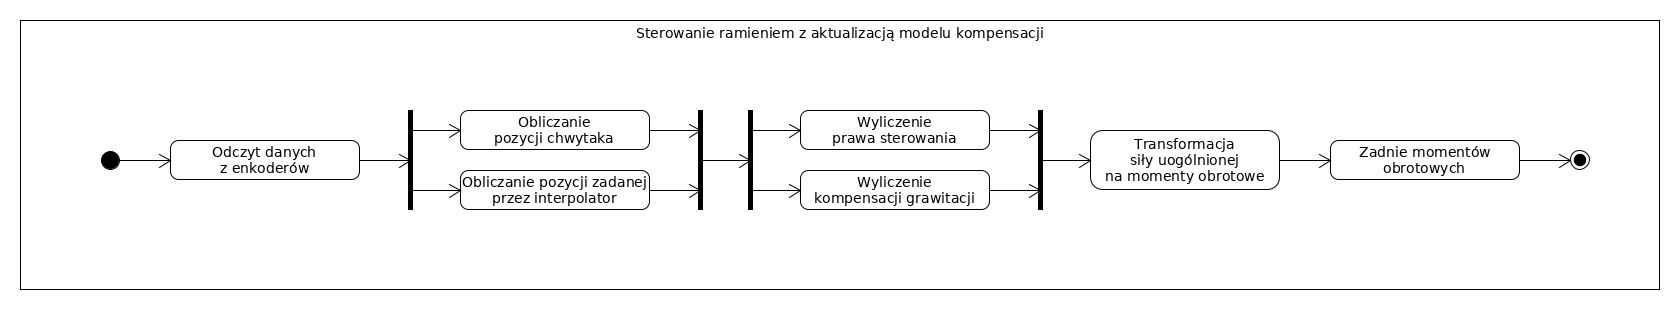
\includegraphics[width=.99\textwidth]{images/kompensacja.png}
	\caption{Diagram aktywności pokazujący przebieg sterowania ramieniem robota.}
	\label{fig:sterowanie}
\end{figure}

Zadany odgórnie model stosowany przy wyliczaniu kompensacji grawitacji ma pewne wady. Jeśli model nie jest dokładny, siła grawitacji nie zostanie skompensowana właściwie. W~trakcie pracy robot zmienia swoje własności np. przez zmianę tarcia związanego ze zmianą temperatury. Dodatkową niedokładność wprowadza zmiana konfiguracji stawów ujętego w~modelu jako jeden człon chwytaka.  Dla rozważań ważniejszy jest fakt, iż jeśli robot chwyci przemiot, którym ma manipulować, to jego parametry nie zostaną uwzględnione w~tym modelu. Spowoduje to, że ramiona robota będą opadać.

\section{Analiza wymagań}
Rozważania dotyczące możliwych rozwiązań ogólnie zarysowanego problemu można usystematyzować. Środowiskiem badawczym jest robot Velma. Przypadki użycia (rys. \ref{fig:usecase}) odzwierciedlają pracę systemu. Algorytm kompensujący grawitację ma działać przez cały czas pracy robota z~podejmowanym przedmiotem. 
\subsection{Przypadki użycia}
Kompensacja grawitacji jest oddzielnym przypadkiem  użycia robota, który rozszerza przypadki użycia systemu w~trakcie pracy w~trybie sterowania impedancyjnego.

\begin{figure}[H]
	\centering
	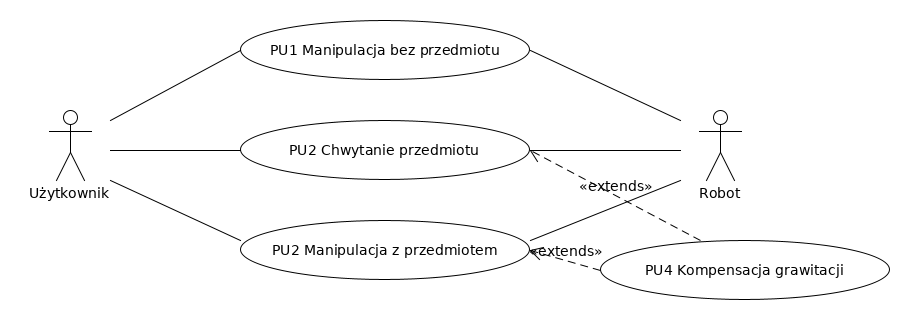
\includegraphics[width=.9\textwidth]{images/usecase.png}
	\caption{Diagram przypadków użycia robota z~uwzględnieniem algorytmu kompensacji grawitacji}
	\label{fig:usecase}
\end{figure}


Aktorami korzystającymi z~systemu są:
\begin{itemize}
	\item \textbf{Robot} - Robot wykonujący zadanie chwycenia przedmiotu.
	\item \textbf{Użytkownik} - System zewnętrzny wydający polecenia.
\end{itemize}


Przypadki użycia to:
\begin{itemize}
	\item \textbf{PU1 Manipulacja bez przedmiotu} - Konfiguracja ramienia robota może się zmieniać lecz robot nie trzyma żadnego przedmiotu. Algorytm kompensacji grawitacji nie powinien zmieniać prawa sterowania. 
	\item \textbf{PU2 Chwytanie przedmiotu} - Robot zaciska chwytak na przedmiocie o~nieznanych parametrach, a~następnie podnosi.  
	\item \textbf{PU3 Manipulacja z~przedmiotem} - Konfiguracja ramienia może się zmieniać, a algorytm kompensacji grawitacji powinien przeciwdziałać sile grawitacji wywieraną na chwytany przedmiot.
	\item \textbf{PU4 Kompensacja grawitacji} - Robot kompensuje siłę grawitacji wywieraną na chwytany przedmiot.
\end{itemize}

\subsection{Wymagania}
Konkretne wymagania dotyczące systemu są podyktowane środowiskiem badawczym oraz potrzebami Zespołu Programowania Robotów i~Systemów Rozpoznających. 
\begin{itemize}
	\item System dostarcza gotowe komponenty potrzebne do pracy ramienia, w~szczególności: generatora trajektorii, interpolatora oraz wyznaczania kinematyki prostej 
	\item System pozyskuje dane o~otoczeniu na podstawie odczytów z~czujników położenia stawów.
	\item System samodzielnie kompensuje siłę grawitacji związaną z~masą wszystkich członów robota.
	\item Parametry chwytanego obiektu związane z~masą i inercją nie są znane i~mogą być zmienne w~czasie.
\end{itemize}

\subsection{Zarys rozwiązania}
Przedstawione wymagania pozwalają na wyspecyfikowanie założeń dotyczących modyfikacji oprogramowania robota. Algorytm kompensacji grawitacji musi wyliczać dodatkowy moment w~stawach robota. Do momentów obrotowych wyliczanych na postawie  prawa sterowania impendancyjnego w~przestrzeni operacyjnej robota należy dodać te związane z~kompensacją masy przedmiotu.
\begin{itemize}
	\item Algorytm kompensacji grawitacji zostanie dodany do komponentu odpowiedzialnego za wyliczanie prawa sterowania impedancyjnego.
	\item Trajektoria końcówki ramienia powinna być zbliżona do trajektorii zadanej.
	\item Algorytm kompensacji nie może zaburzać cech sterowania impedancyjnego pozwalających na uginanie się robota w~momencie kolizji.
\end{itemize}


\section{Rozwiązania}

Najprostszym rozwiązaniem jest poznanie masy przedmiotu poprzez odczyt siły grawitacji z~czujnika siły zamieszczonego w~chwytaku, a~następnie dodanie wartości tej siły o~przeciwnym znaku do prawa sterowania. Takie rozwiązanie nie jest dość dokładne. Na pomiar siły mają wpływ inne siły niż siła grawitacji i~znacznie zaburzają wynik. Istnieje potrzeba znalezienia innego rozwiązania.

Pierwsze z rozwiązań, oparte na dodaniu do istniejącego prawa sterowania członu całkującego, jest proste w~implementacji lecz prawdopodobnie nie jest zbyt dokładne. Nie pozwala na poznanie żadnych parametrów przedmiotu, który jest chwytane. Drugie z rozwiązań, zakładające obliczenie parametrów modelu przedmiotu, jest skomplikowane w~implementacji i~wymaga większych zasobów obliczeniowych. Stanowi to realny problem w~systemie czasu rzeczywistego. 

\subsection{Rozwiązanie oparte na regulatorze PID}
\label{chap:rozw_pid}
Opadanie ramion można interpretować jako błąd pomiędzy pozycją zadaną przez interpolator i~pozycją zadaną czyli uchyb. Problem uchybu rozwiązuje regulator PID opisany w~sekcji \ref{chap:key}. Jego zastosowanie rodzi ryzyko, że ramiona robota usztywnią się i będą powodować uszkodzenia w~trakcie kolizji. Stąd wniosek aby połączyć prawo sterowania impedancyjengo i~regulator PID w~nowe prawo sterowania \cite{bib:gravity2, bib:rozw_pid1}. Po połączeniu obydwu praw sterowania i~zastosowaniu ograniczenia całkowania, ramiona nie powinny być nadmiernie sztywne. 

Niektóre człony są takie same w~zaprezentowanych prawach sterowania. W~impedancyjnym prawie sterowania nie ma członu całkującego i~został on wzięty z~algorytmu PID. W~rezultacie nowe prawo sterowania jest postaci (rys. \ref{fig:pid_schemat}):

\begin{equation}
\label{eq:prawo_ster}
\boldsymbol{\mathcal{F}} = \boldsymbol{K_x}\boldsymbol{e_x} + \boldsymbol{D_x}\dot{\boldsymbol{e_x}} + \int_{0}^{t}  \boldsymbol{I_x}\boldsymbol{e_x}dt
\end{equation}

gdzie:
\begin{itemize}
	\item $\boldsymbol{\mathcal{F}}$ to wektor sił wynikowych
	\item $\boldsymbol{K_x}$ to diagonalna macierz sprężystości
	\item $\boldsymbol{D_x}$ to diagonalna macierz sztywności
	\item $\boldsymbol{I_x}$ to diagonalna macierz członu całkującego
	\item $\boldsymbol{e_x}$ to wektor uchybu
\end{itemize}

Parametry członu całkującego powinny mieć na tyle małe wartości, by 
nie zdominowały używanego wcześniej prawa sterowania impedancyjnego, a~jedynie poprawiały jego działanie. Ważne jest też zastosowanie ograniczenia całkowania. Po wyliczeniu prawa sterowania należy zastosować przekształcenie obliczające momenty obrotowe, które mają być zadane na silniki robota analogicznie do procedury pokazanej w~sekcji \ref{chap:jakobian}. 

\begin{figure}
	\centering
	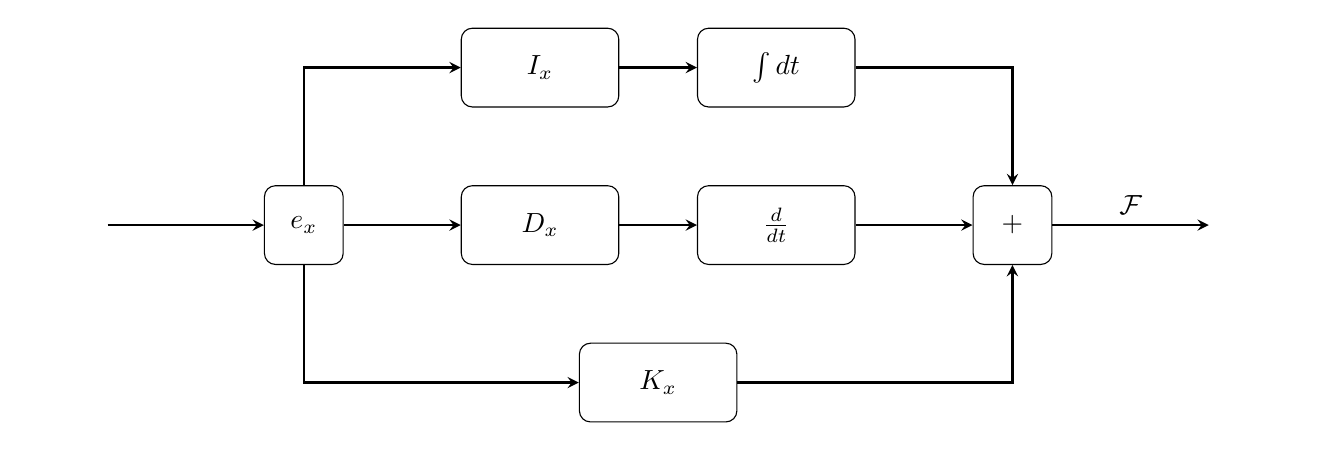
\begin{tikzpicture}[node distance=2cm]
	\tikzstyle{block} = [rectangle, rounded corners, minimum width=2cm, minimum height=1cm, text centered, draw=black, fill=white!30];
	\tikzstyle{sumator} = [rectangle, rounded corners, minimum width=1cm, minimum height=1cm, text centered, draw=black, fill=white!30];
	\tikzstyle{sumwhite} = [rectangle, rounded corners, minimum width=1cm, minimum height=1cm, text centered, draw=white, fill=white!30];
	\tikzstyle{arrow} = [thick,->,>=stealth];
	\node (integral0) [block] {$\boldsymbol{I_x}$};
	\node (integral1) [block, right of=integral0, xshift=1cm] {$\boldsymbol{\int dt}$};
	\node (dot0) [sumator, below of=integral0, xshift=-3cm] {$\boldsymbol{e_x}$};
	\node (dot3) [sumwhite, right of=dot0, xshift=-5cm] {};
	\node (deriv0) [block, below of=integral0] {$\boldsymbol{D_x}$};
	\node (deriv1) [block, right of=deriv0, xshift=1cm] {$\boldsymbol{\frac{d}{dt}}$};
	\node (prop0) [block, below of=deriv0, xshift=1.5cm] {$\boldsymbol{K_x}$};
	\node (dot1) [sumator, right of=deriv1, xshift=1cm] {$\boldsymbol{+}$};
	\node (dot2) [sumwhite, right of=dot1, xshift=1cm] {};
	
	\draw [arrow] (integral0) -- (integral1);
	\draw [arrow] (deriv0) -- (deriv1);
	\draw [arrow] (dot0) |- (integral0);
	\draw [arrow] (dot0) -- (deriv0);
	\draw [arrow] (dot0) |- (prop0);
	\draw [arrow] (integral1) -| (dot1);
	\draw [arrow] (deriv1) -- (dot1);
	\draw [arrow] (prop0) -| (dot1);
	\draw [arrow] (dot1) -- node[anchor=south] {$\boldsymbol{\mathcal{F}}$} (dot2);
	\draw [arrow] (dot3) -- (dot0);
	\end{tikzpicture}
	\caption{Schemat nowego prawa sterowania z elementami prawa sterowania impedancyjnego i regualatora PID. }
	\label{fig:pid_schemat}
\end{figure}

\section{Rozwiązanie oparte na estymacji modelu robota}
\label{chap:rozw_model}
Problem można również rozwiązać poprzez estymację nowego modelu, wykorzystywanego do kompensacji grawitacji w postaci takiej jak w~sekcji \ref{chap:estymacja}, ale rozszerzonego o~zastosowane prawo sterowania \cite{bib:rozw_opt1, bib:rozw_opt2} (rys. \ref{fig:kompensacja}). Równanie siły uogólnionej dla chwili $i$ jest wtedy postaci:
\begin{equation}
\boldsymbol{\mathcal{F}_{m}}_i = \boldsymbol{K_x}\boldsymbol{e_x} + \boldsymbol{D_x}\dot{\boldsymbol{e_x}} + \boldsymbol{\Lambda}(\boldsymbol{q})\boldsymbol{\ddot{x}} + \boldsymbol{\mu}(\boldsymbol{x}, \boldsymbol{\dot{x}}) + \boldsymbol{\gamma}(\boldsymbol{q}) + \boldsymbol{\eta}(\boldsymbol{q}, \boldsymbol{\dot{q}})
\end{equation}

gdzie: 

\begin{itemize}
	\item $\boldsymbol{\Lambda}$ to dodatnio określona macierz inercji w~przestrzeni zadań
	\item $\boldsymbol{\mu}$ to macierz sił Coriolisa i~sił odśrodkowych	
	\item $\boldsymbol{\gamma}$ to wektor sił grawitacji
	\item $\boldsymbol{\eta}$ to macierz sił tarcia oraz nieuwzględnionych sił
	\item $\boldsymbol{q}$ to wektor położeń stawów w~przestrzeni konfiguracyjnej
	\item $\boldsymbol{x}$ to wektor położeń końcówki w~przestrzeni zadań
	\item $\boldsymbol{K_x}$ to diagonalna macierz sprężystości
	\item $\boldsymbol{D_x}$ to diagonalna macierz sztywności
	\item $\boldsymbol{e_x}$ to wektor uchybu
\end{itemize} 


Czujnik skrętnika sił dla każdej chwili $i$ pozwala na odczytanie rzeczywistego wektora siły uogólnionej w~końcówce $\boldsymbol{\mathcal{F}}_i$. Dzięki temu możemy uzyskać różnicę pomiędzy tymi dwoma wartościami:
\begin{equation}
\boldsymbol{\mathcal{F}_{e}}_i = \boldsymbol{\mathcal{F}}_{i} - \boldsymbol{\mathcal{F}_{m}}_i
\end{equation}
a następnie zastosować optymalizację, której parametrami są macierze stosowane do wyliczania modelu. Problem optymalizacji powinien być oparty o~minimalizację różnicy dla $n$ próbek:
\begin{equation}
\begin{aligned}
& \underset{\boldsymbol{\Lambda}(\boldsymbol{q})\boldsymbol{\ddot{x}}, \boldsymbol{\mu}(\boldsymbol{x}, \boldsymbol{\dot{x}}), \boldsymbol{\gamma}(\boldsymbol{q}), \boldsymbol{\eta}(\boldsymbol{q}, \boldsymbol{\dot{q}})}{\text{min}}
& & \sum_{i = 1}^{n} || \boldsymbol{\mathcal{F}_{e}}_i ||
\end{aligned}
\end{equation}

W trakcie praktycznych obliczeń można stosować pewne uproszczenia modelu. Przy założeniu braku ruchu pomiędzy chwytanym przedmiotem a~chwytakiem możemy potraktować ten przedmiot jako część chwytaka. W~takiej sytuacji dodanie przedmiotu do chwytaka powoduje zmianę parametrów środka ciężkości masy oraz ostatniego członu i~wprowadza zmiany tylko z~tym związane. Można też przyjąć pewne uproszczenia wynikające z~faktu, że chwytany przedmiot ma stosunkowo małą masę w porównaniu z~masą całego ramienia robotycznego. Estymowany model powinien być aktualizowany na bieżąco w~trakcie pracy robota i~stosowany w~celu kompensacji grawitacji zamiast pierwotnego modelu.

Optymalizacja nieliniowa jest rozwiązywana na tyle wolno, że model nie może być aktualizowany tak często jak cały system sterowania robota. Rozwiązanie jest też dużo trudniejsze w~implementacji niż opisane w~sekcji \ref{chap:rozw_pid}. 

\begin{figure}
	\centering
	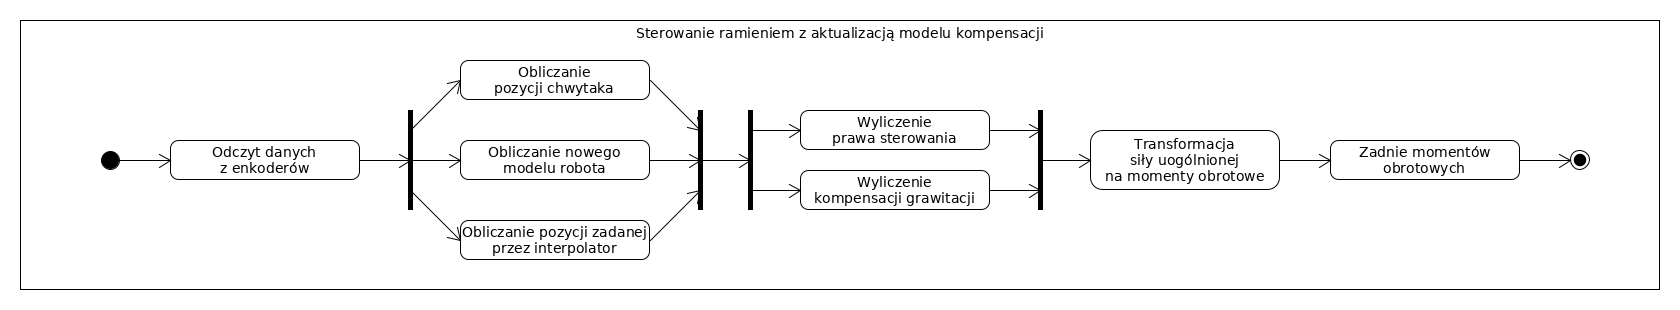
\includegraphics[width=.99\textwidth]{images/komp_model.png}
	\caption{Diagram aktywności pokazujący przebieg sterowania ramieniem robota z~aktualizacją modelu.}
	\label{fig:kompensacja}
\end{figure}

\subsection{Wybór rozwiązania}

Implementacja rozwiązania z~sekcji \ref{chap:rozw_model} rodzi sporo problemów. W~praktyce trudne jest zbudowanie odpowiedniego zadania optymalizacji, które zagwarantuje na tyle dobry model, by grawitacja była odpowiednio kompensowana. Optymalizacja obliczana jest na tyle wolno, że nie ma możliwości umieszczenia estymatora modelu jako jednego z~komponentów podsystemu sterowania \textit{velma\_core\_cs}. Komponent musiałby zostać umieszczony w~nowym agencie, który pracuje z~mniejszą niż cały system częstotliwością i~komunikuje się z~systemem robota za pośrednictwem interfejsu ROSa. W~początkowej fazie, gdy przedmiot zostanie chwycony ramiona robota zostają najczęściej nieruchome. Grawitacja chwyconego narzędzia nie jest kompensowana. Estymacja modelu jest wtedy wyjątkowo niedokładna. W~początkowej fazie należałoby stosować uproszczony model tylko po to, by robot mógł podnieść przedmiot. Dopiero po kilku ruchach, gdy zadanie optymalizacji zostanie poprawnie rozwiązane, można wprowadzić właściwy model z~użyciem narzędzi logiki rozmytej.

Wspomniane wady były podstawą decyzji o~implementacji rozwiązania z~sekcji \ref{chap:rozw_pid}. Główną wadą jest niemożność wyekstrahowania danych dotyczących przedmiotu, który chwyta robot. Kolejną wadą może być lekkie usztywnienie stawów, co nie powinno mieć dużego znaczenia. W~sterowaniu impedancyjnym w~przestrzeni operacyjnej wirtualna sprężyna jest zawieszona pomiędzy chwytakiem a~punktem zadanym, a~nie w~konkretnych stawach robota. Do tego zakładamy niskie współczynniki członu całkującego.








